
\section{Ejercicio 8 (Migración vs. No Migración)}
Con el objetivo de comparar el scheduling round robin con y sin migracion de nucleos, se realizaron distintas experimentaciones con distintos costos de cambio de contexto, de migración de núcleo, cantidad de núcleos, el quantum de cada uno y duración de quantum para cada cpu.

Con el objetivo de simplificar la experimentción algunos parámetros se dejaron fijos, estos fueron elejidos porque no producen un efecto sobre el resultado al variar, teniendo o no teniendo migración activada. En particular los parámetros que se dejaron fijos en este caso fueron el costo de context switch, que no afecta el resultado ya que con o sin migración se realizan la misma cantidad de context switch's.

Primero se muestran los resultados para tiempo de migración = 1, dos nucleos, para 4 tareas.
\begin{figure}[h]
  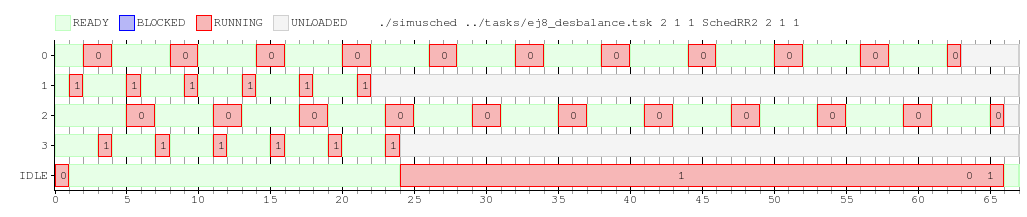
\includegraphics[width=\textwidth]{ej8/figs/sinMigracion.jpg}
  \caption{Diagramas de Gantt sin migración.}
\end{figure}


\begin{figure}[h]
  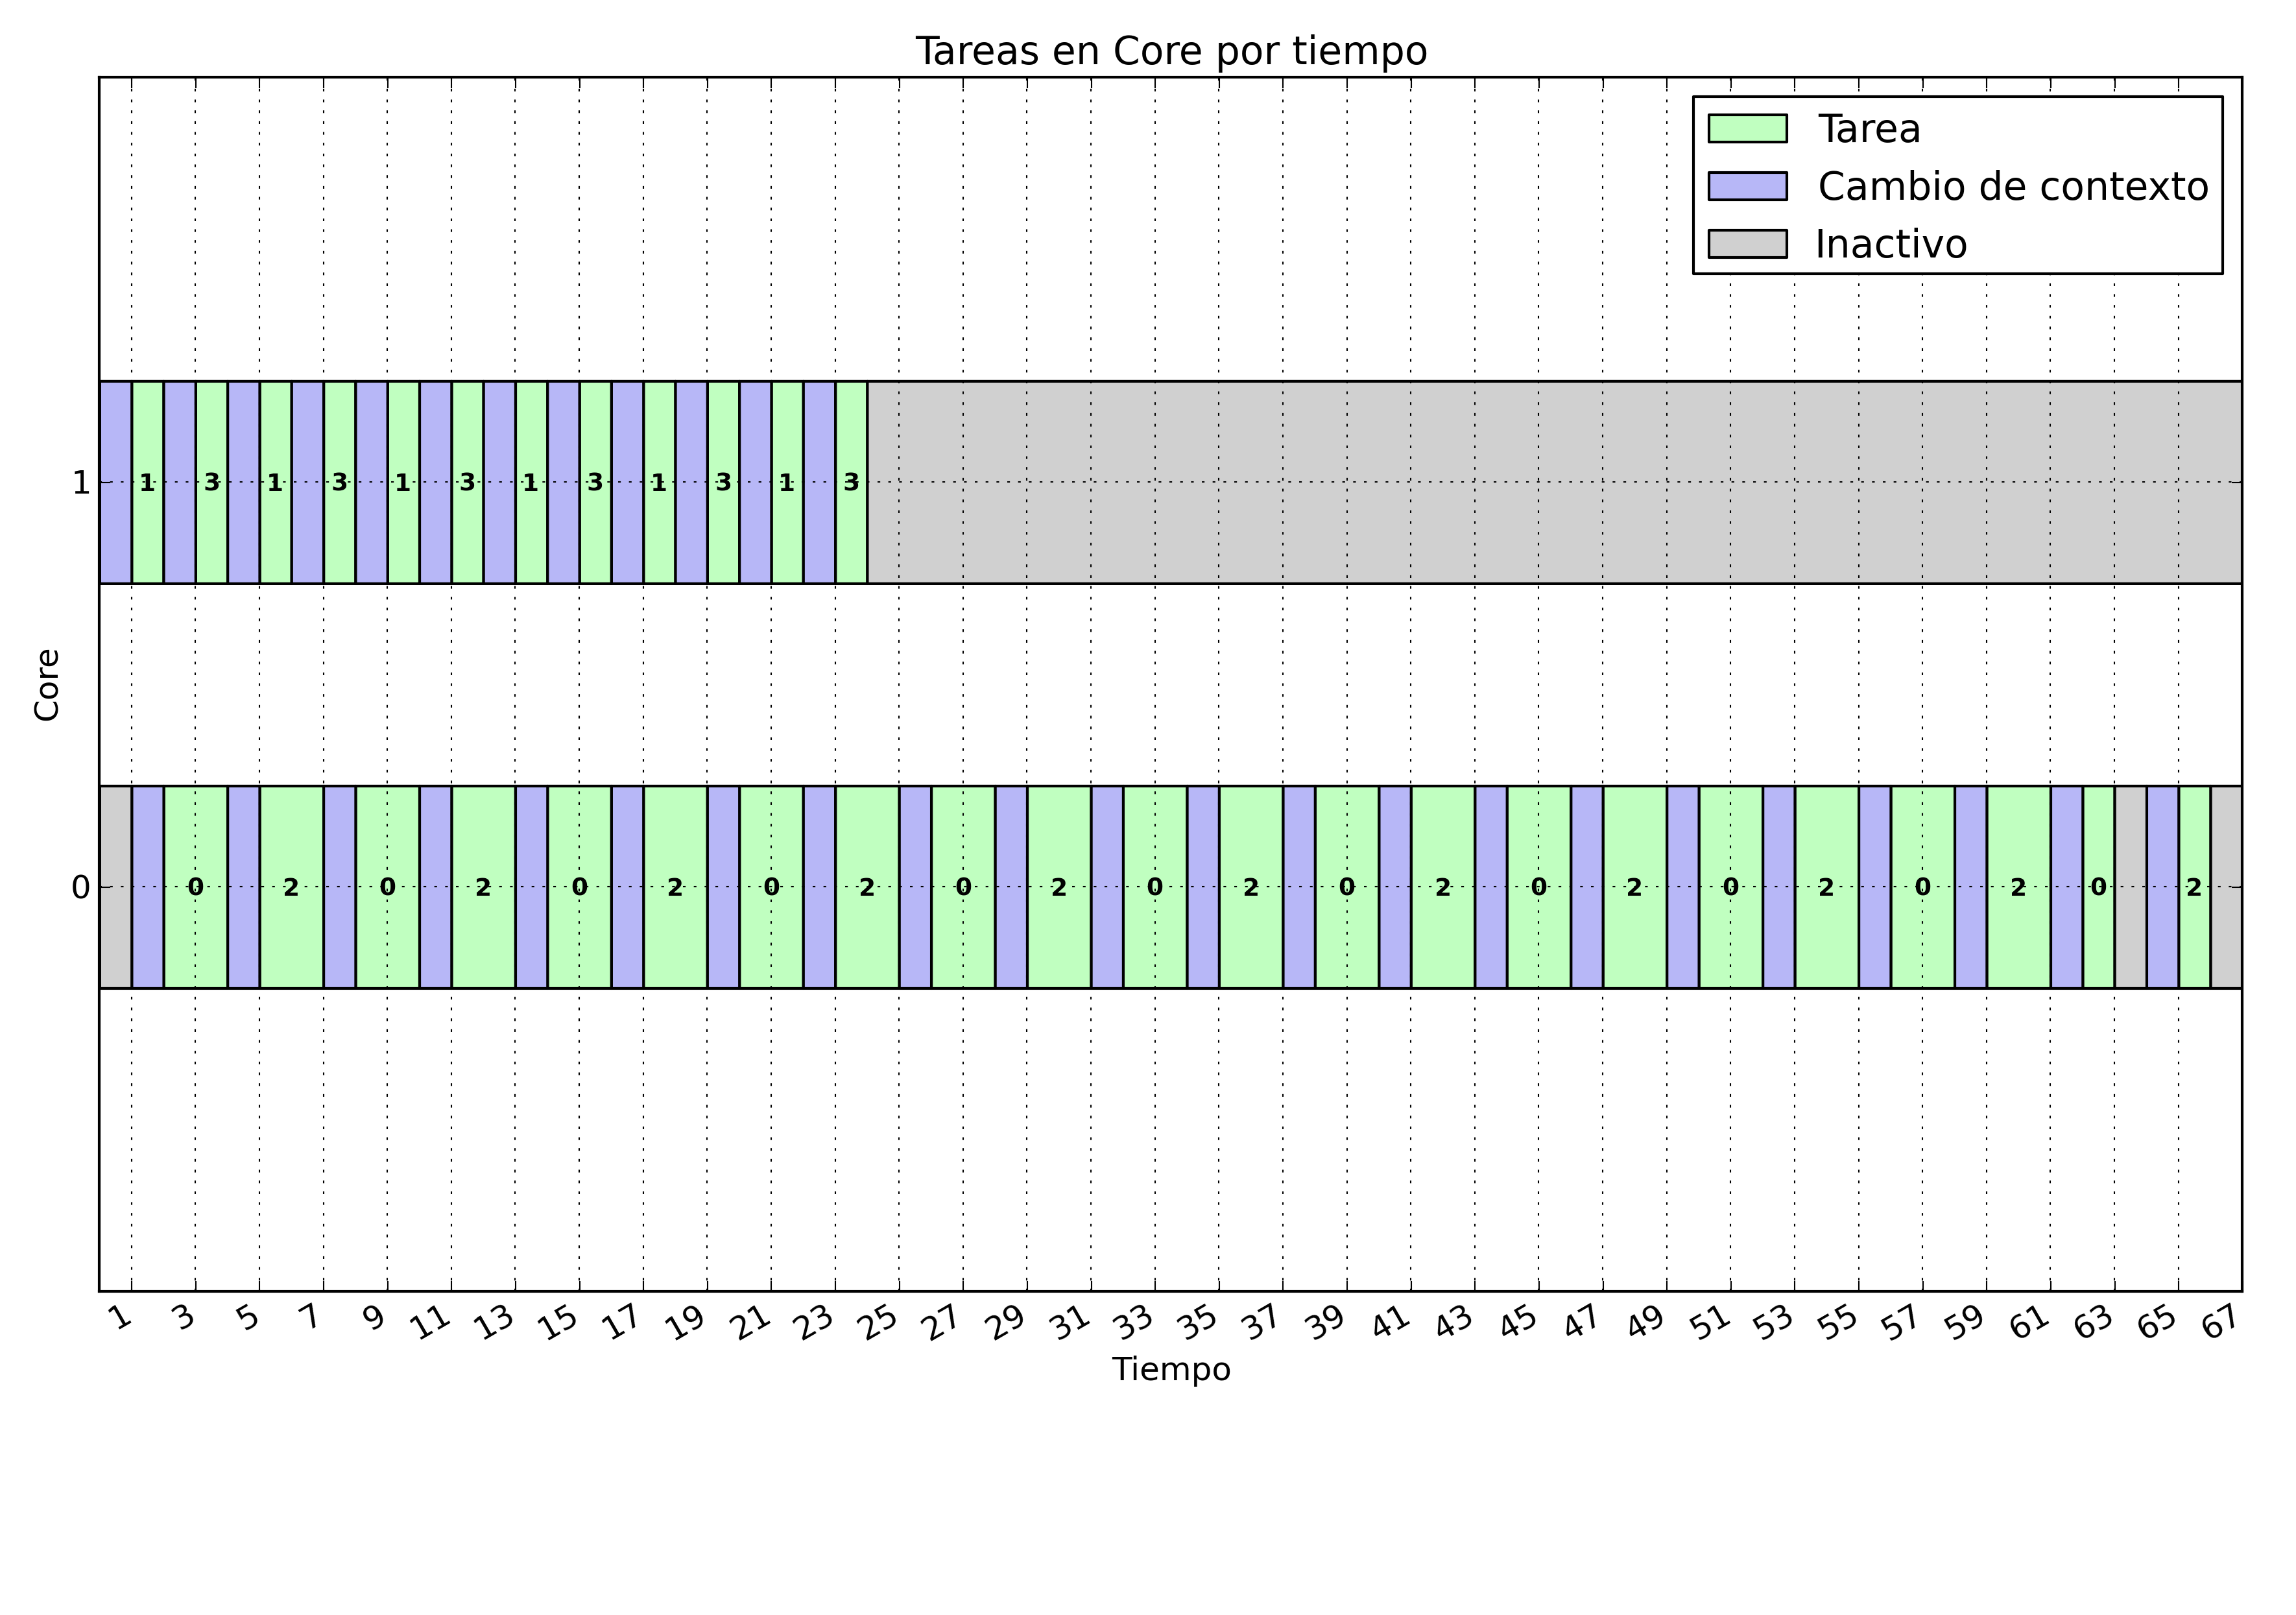
\includegraphics[width=\textwidth]{ej8/figs/coresSinMigracion.png}
  \caption{Diagramas de procesadores sin migración.}
\end{figure}


\begin{figure}[h]
  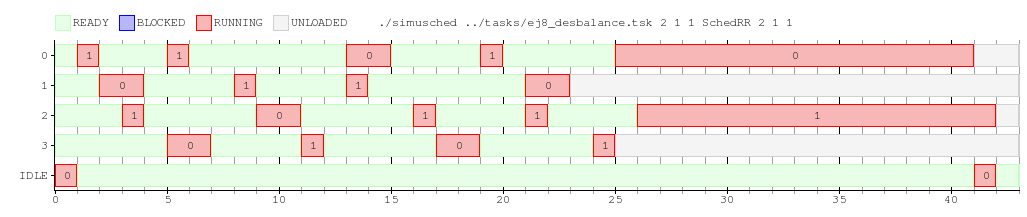
\includegraphics[width=\textwidth]{ej8/figs/conMigracion.jpg}
  \caption{Diagramas de Gantt con migración.}
\end{figure}


\begin{figure}[h]
  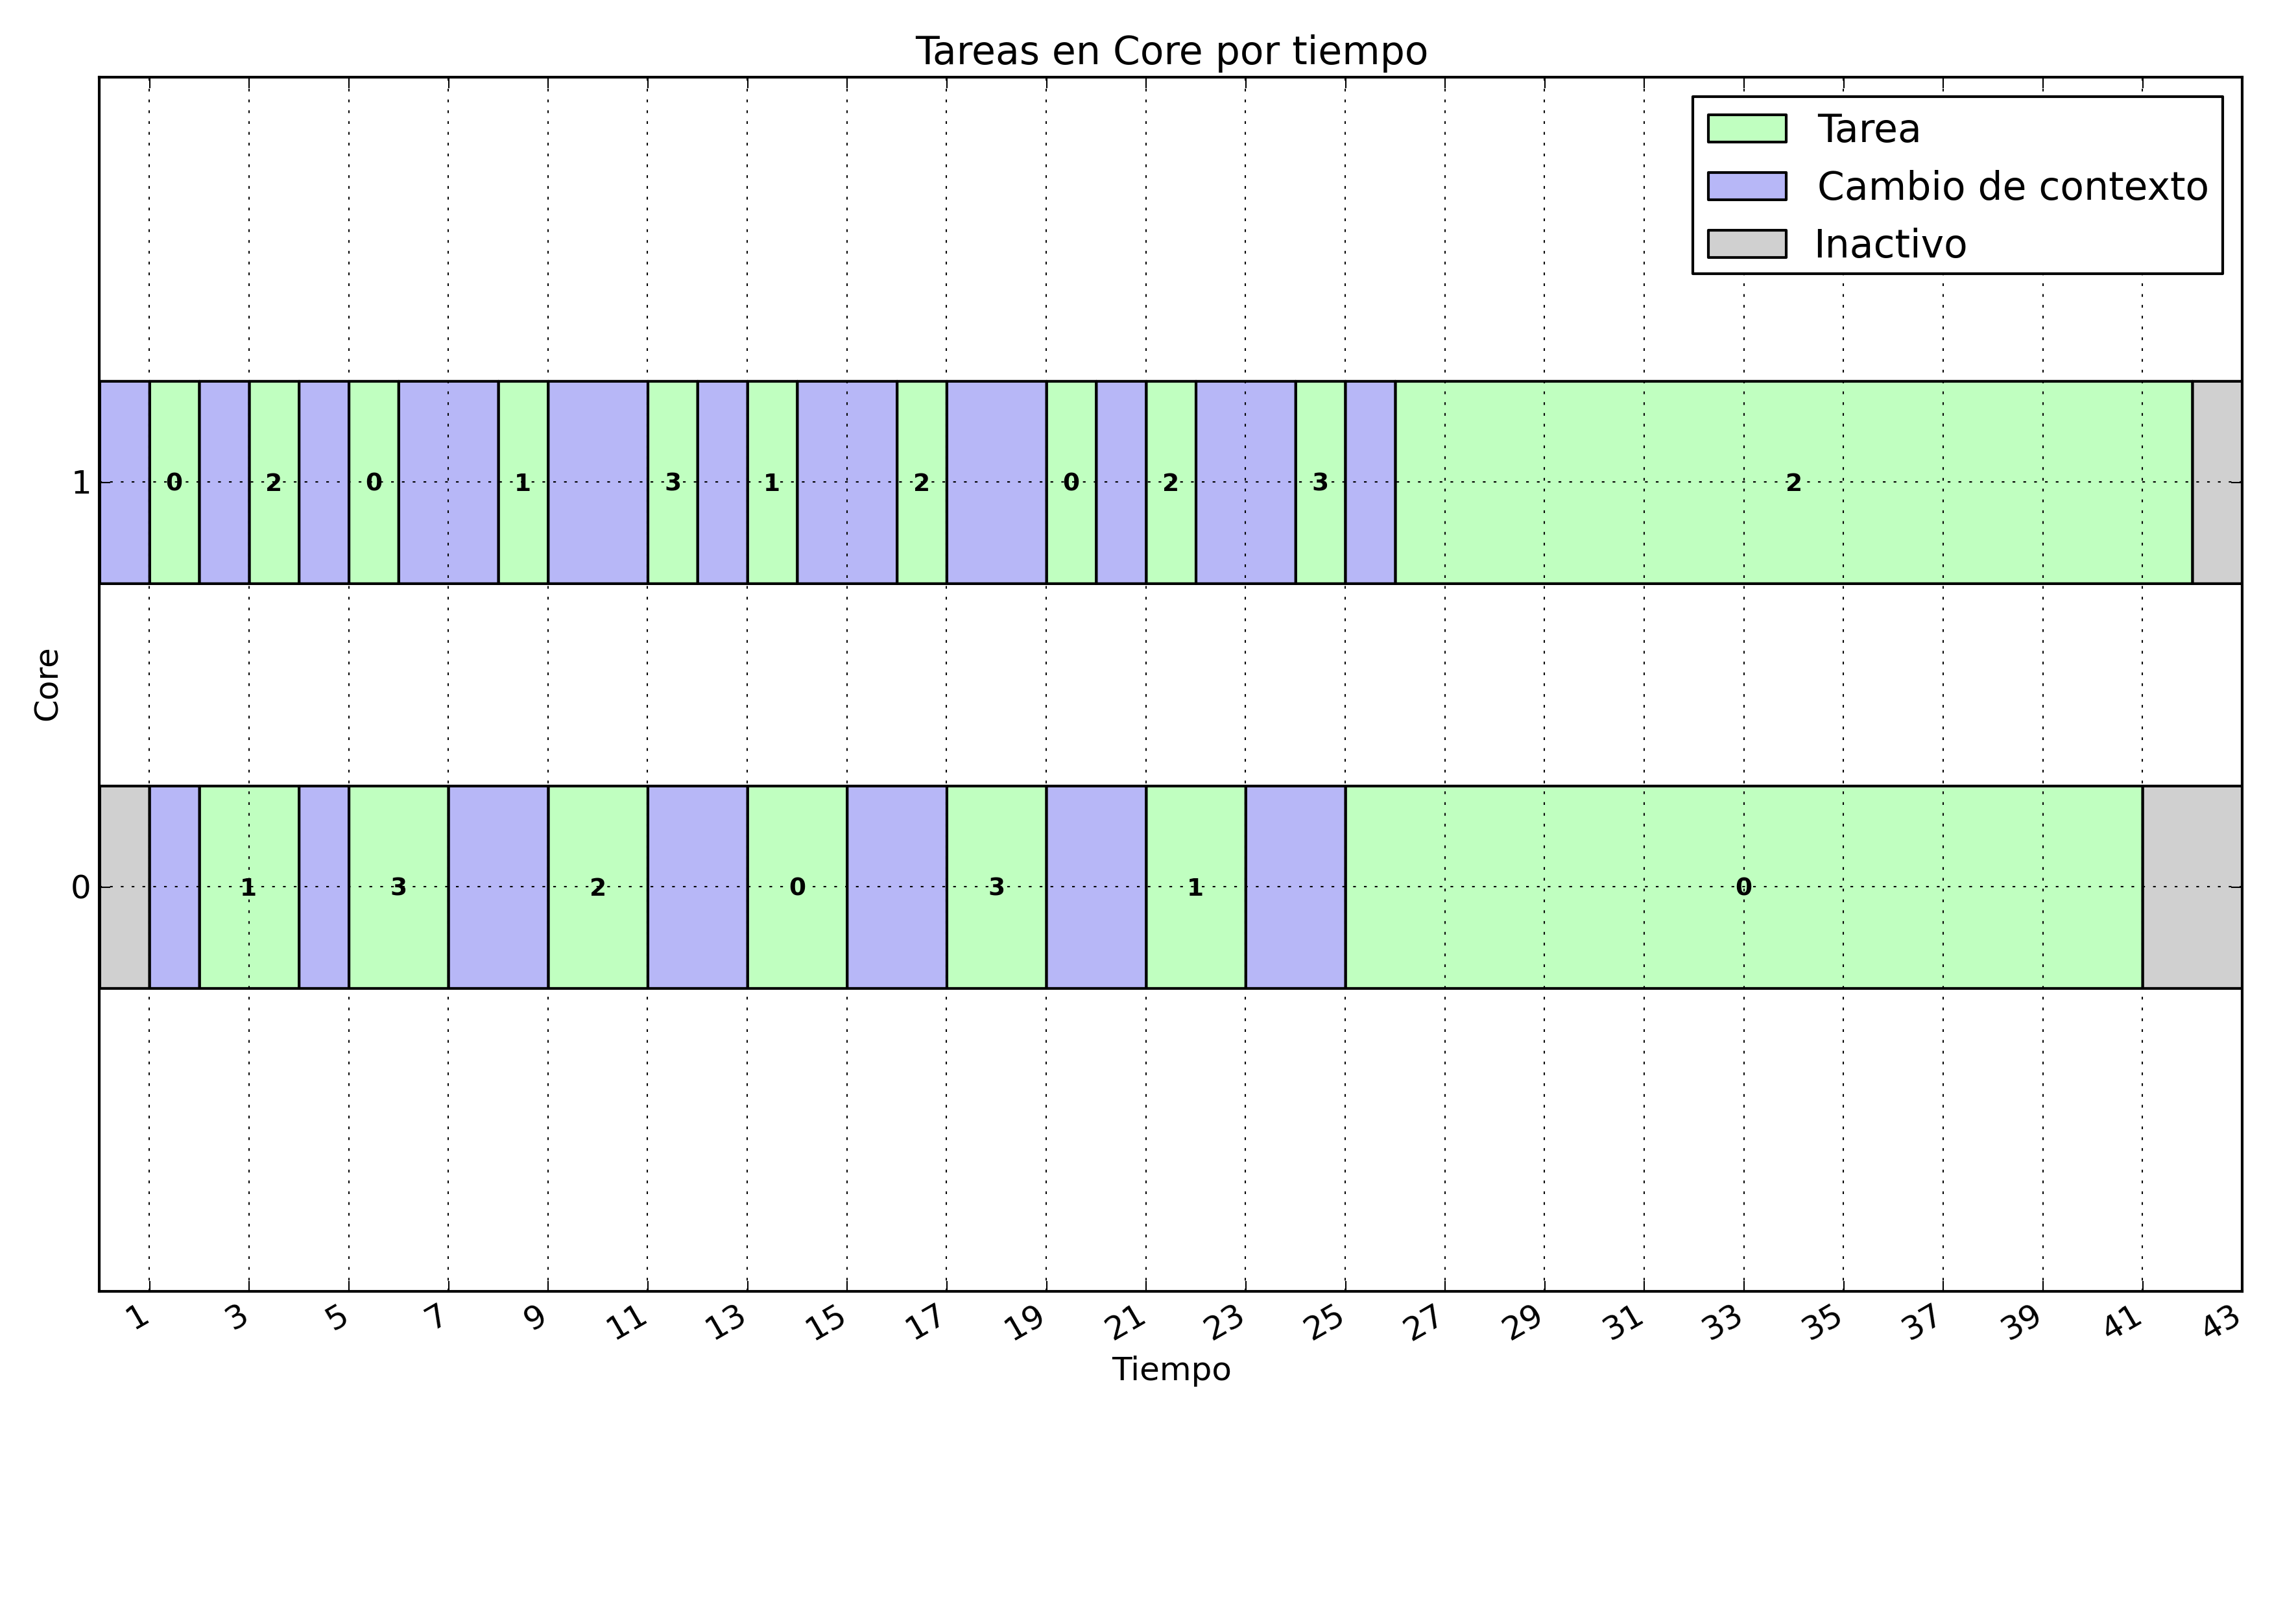
\includegraphics[width=\textwidth]{ej8/figs/coresConMigracion.png}
  \caption{Diagramas de procesadores con migración.}
\end{figure}

Como puede observarse mediante la activación de la migración se redujo el tiempo total de ejecución de 66 a 42 ticks.

Se consiguieron posteriormente resultados para distintas cantidades de tareas y nucleos. En todos los casos se obtuvo un resultado similar. En general, las corridas con migración mostraron un mayor tiempo de ejecución que las corridas sin migración. Se observó que en el caso de las corridas con migración se realizaban muchas migraciones que no daba utilidad alguna, y que consumían tiempo. En el caso en que no habia migraciones, se notaba que llegando al final de la ejecucion, uno o varios nucleos permanecian inactivos, mientras que otros trabajaban en varias tareas. Si bien esto no es óptimo porque hay procesadores ociosos a los que  podrían migrarse tareas, en base a nuestros resultados podemos concluir que en el caso general el beneficio de no gastar tiempo migrando suele superar este problema.

Se condujeron también experimentaciones variando los quantums de los núcleos. Se espera que en el caso de las migraciones, el tener quantums más grandes aporte beneficios extra comparando con el caso no migrante, ya que solo unas pocas migraciones son necesarias, al momento de tener procesadores ociosos, y tener muchas migraciones antes de eso alarga la ejecución.

\begin{figure}[H]
  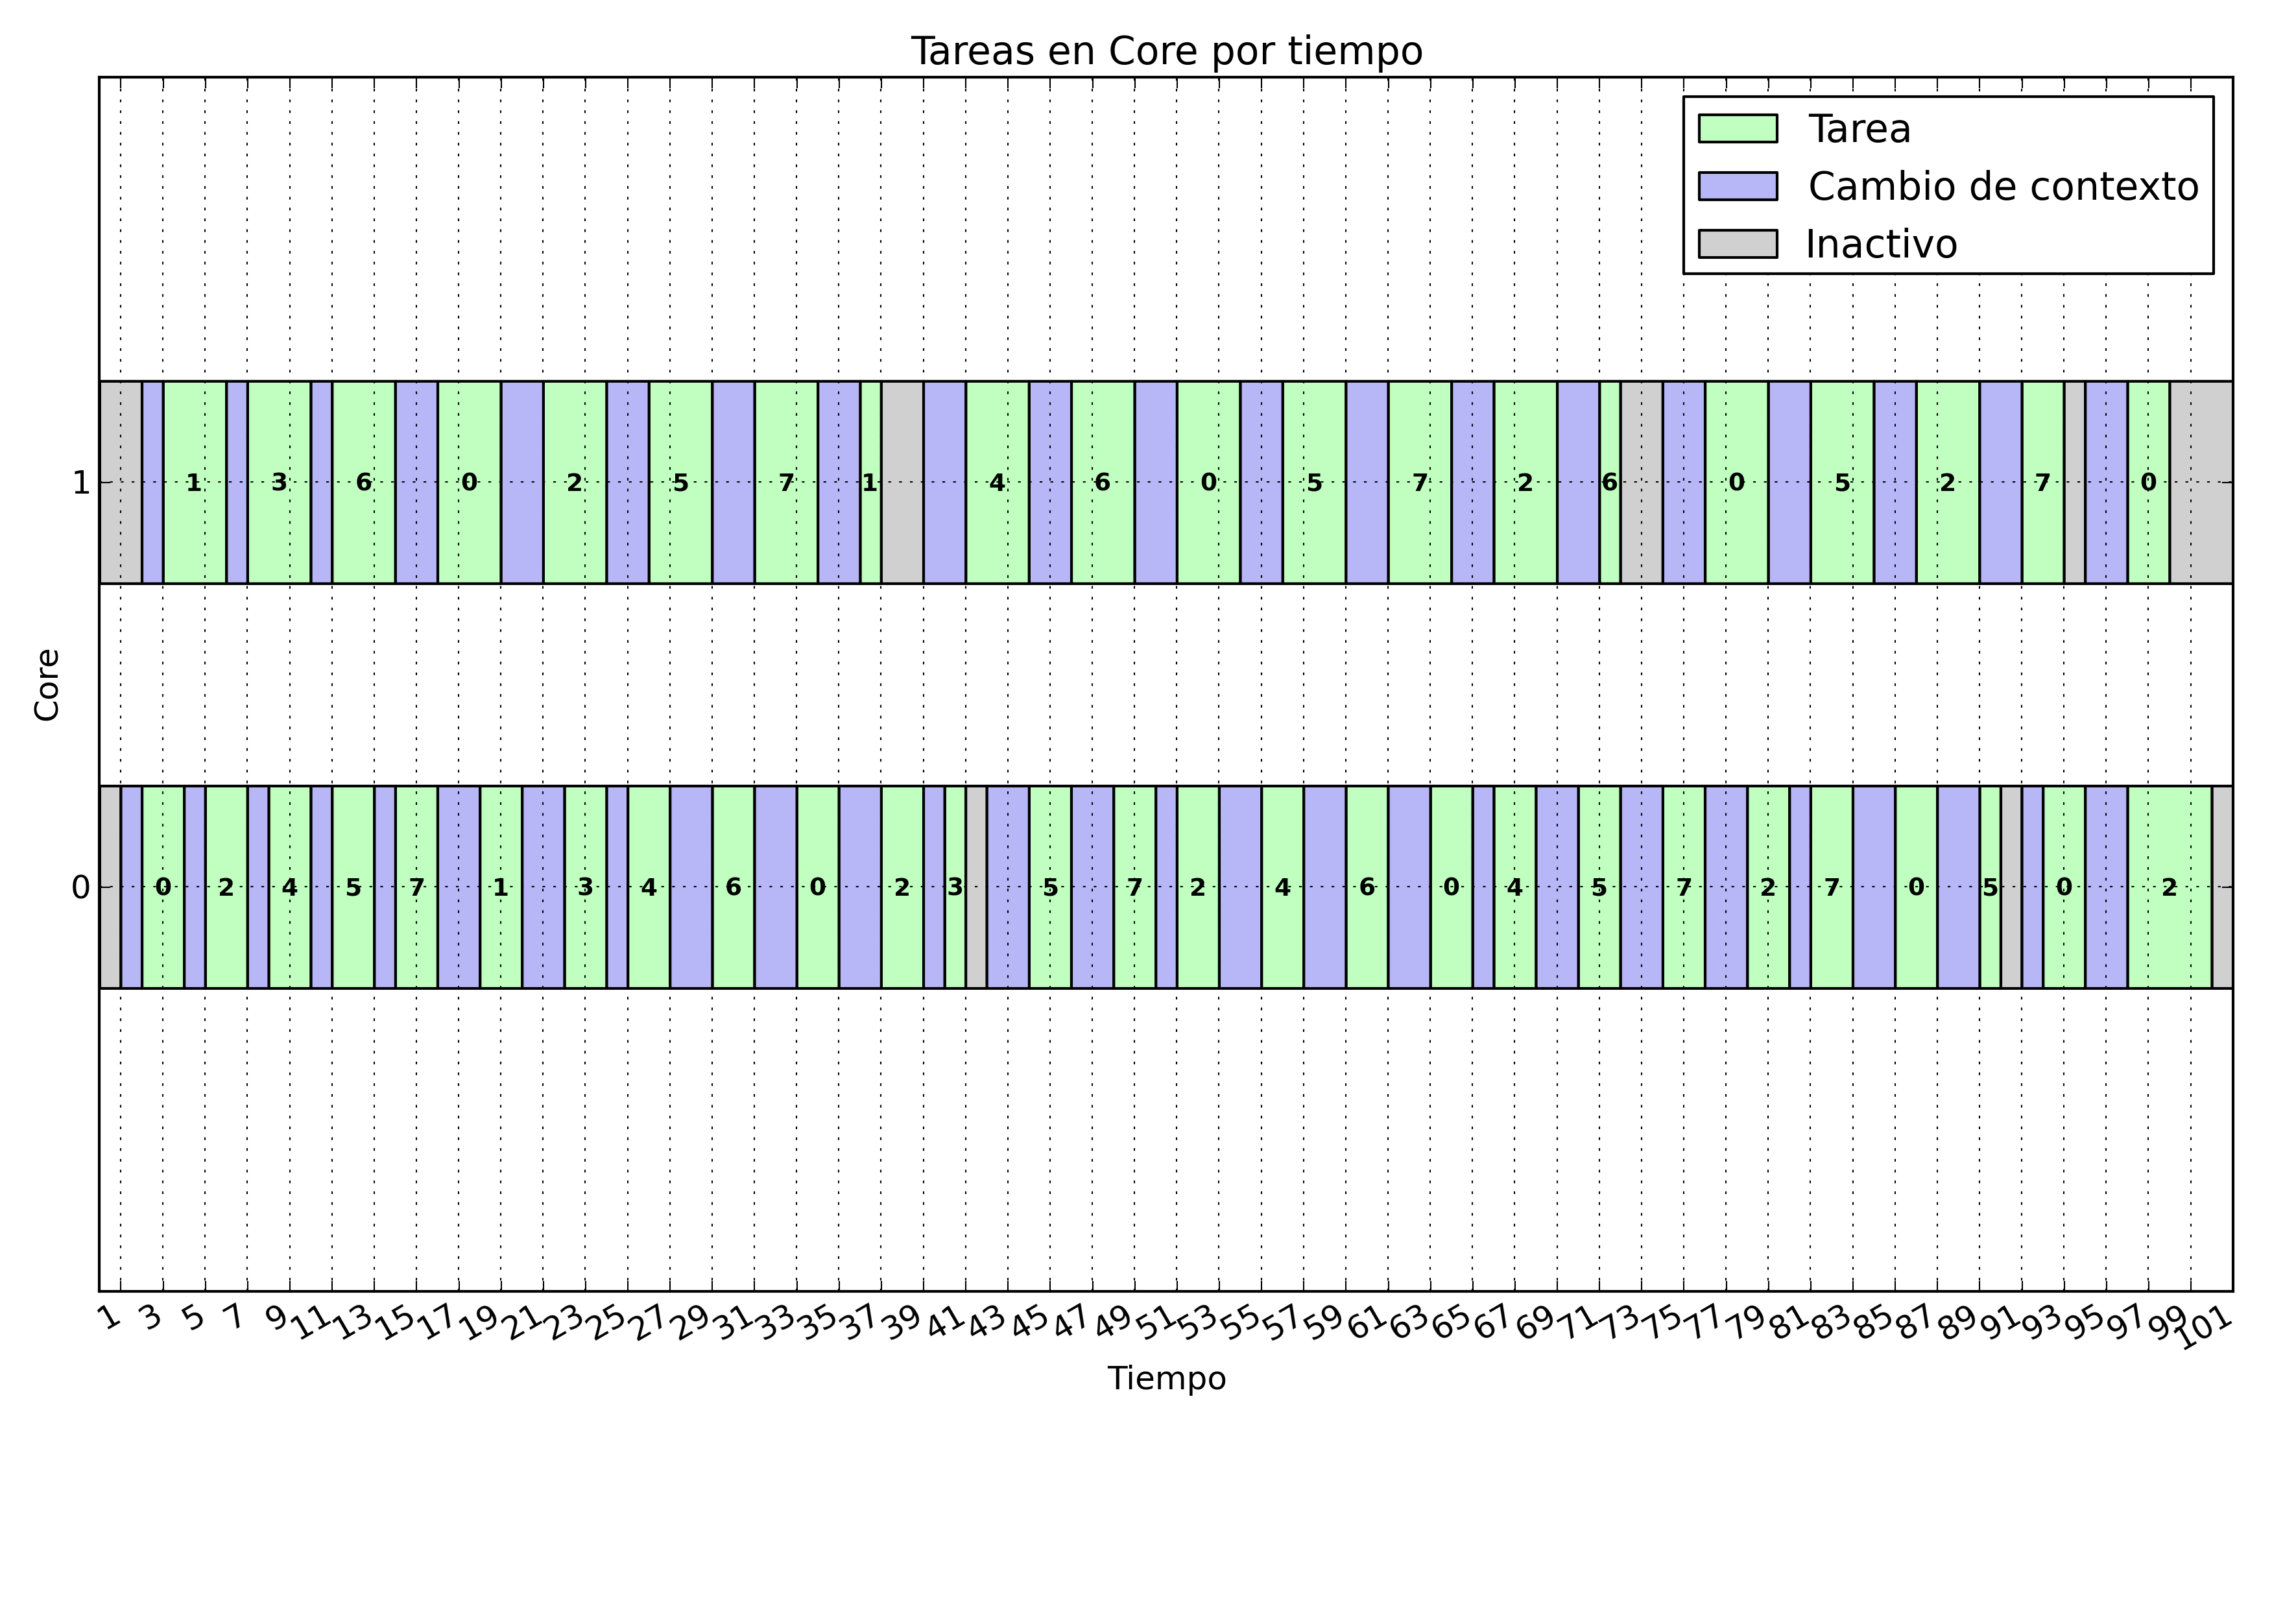
\includegraphics[width=\textwidth]{ej8/figs/C2Q3conMigracion.png}
  \caption{Diagramas de procesadores con migración.}
\end{figure}

\begin{figure}[H]
  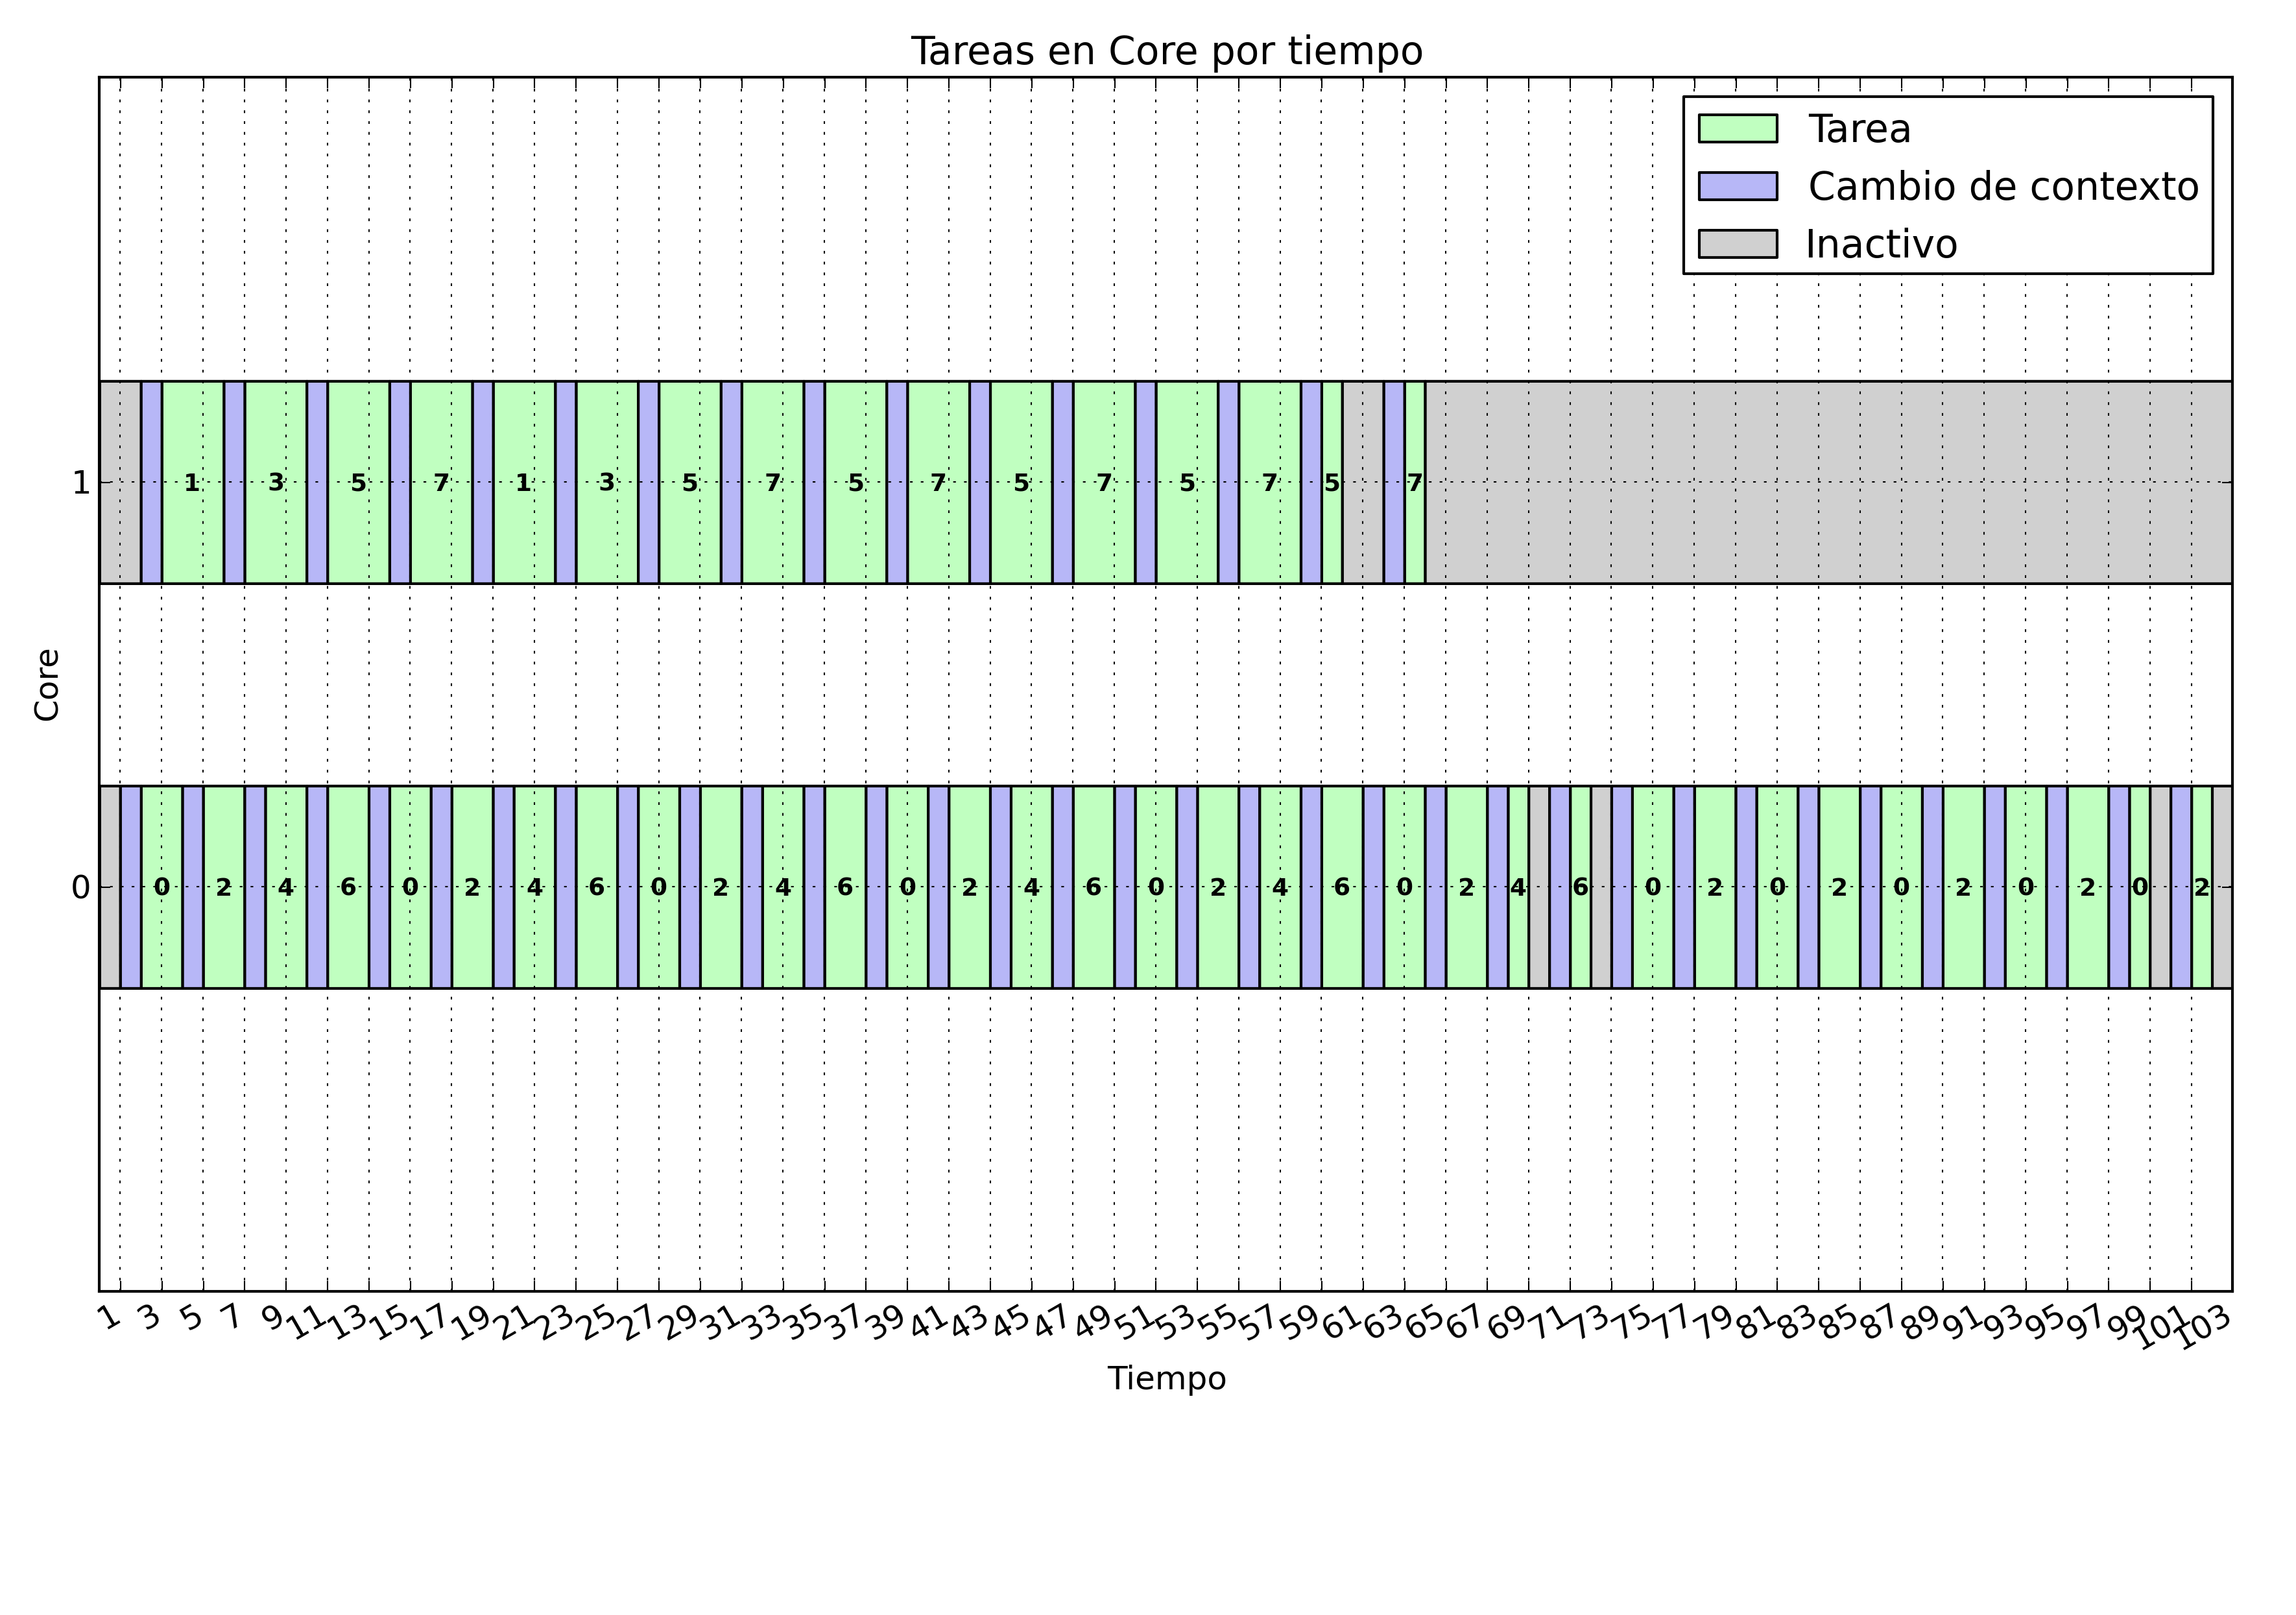
\includegraphics[width=\textwidth]{ej8/figs/C2Q3sinMigracion.png}
  \caption{Diagramas de procesadores sin migración.}
\end{figure}

Como se ve en los gráficos, el resultado confirma la hipótesis propuesta. Efectivamente, la reducción en el tiempo de ejecución fue mayor en el caso del scheduler con migración.

Por último, consideramos que variar el costo de migración entre los núcleos, solo podría extender el tiempo de ejecución en el scheduler con migración. Dado que no causa ningun otro efecto relevante en comparación, no se realizó experimentación de este caso.


